\documentclass[11pt,preprint, authoryear]{elsarticle}

\usepackage{lmodern}
%%%% My spacing
\usepackage{setspace}
\setstretch{1.2}
\DeclareMathSizes{12}{14}{10}{10}

% Wrap around which gives all figures included the [H] command, or places it "here". This can be tedious to code in Rmarkdown.
\usepackage{float}
\let\origfigure\figure
\let\endorigfigure\endfigure
\renewenvironment{figure}[1][2] {
    \expandafter\origfigure\expandafter[H]
} {
    \endorigfigure
}

\let\origtable\table
\let\endorigtable\endtable
\renewenvironment{table}[1][2] {
    \expandafter\origtable\expandafter[H]
} {
    \endorigtable
}


\usepackage{ifxetex,ifluatex}
\usepackage{fixltx2e} % provides \textsubscript
\ifnum 0\ifxetex 1\fi\ifluatex 1\fi=0 % if pdftex
  \usepackage[T1]{fontenc}
  \usepackage[utf8]{inputenc}
\else % if luatex or xelatex
  \ifxetex
    \usepackage{mathspec}
    \usepackage{xltxtra,xunicode}
  \else
    \usepackage{fontspec}
  \fi
  \defaultfontfeatures{Mapping=tex-text,Scale=MatchLowercase}
  \newcommand{\euro}{€}
\fi

\usepackage{amssymb, amsmath, amsthm, amsfonts}

\def\bibsection{\section*{References}} %%% Make "References" appear before bibliography


\usepackage[round]{natbib}

\usepackage{longtable}
\usepackage[margin=2.3cm,bottom=2cm,top=2.5cm, includefoot]{geometry}
\usepackage{fancyhdr}
\usepackage[bottom, hang, flushmargin]{footmisc}
\usepackage{graphicx}
\numberwithin{equation}{section}
\numberwithin{figure}{section}
\numberwithin{table}{section}
\setlength{\parindent}{0cm}
\setlength{\parskip}{1.3ex plus 0.5ex minus 0.3ex}
\usepackage{textcomp}
\renewcommand{\headrulewidth}{0.2pt}
\renewcommand{\footrulewidth}{0.3pt}

\usepackage{array}
\newcolumntype{x}[1]{>{\centering\arraybackslash\hspace{0pt}}p{#1}}

%%%%  Remove the "preprint submitted to" part. Don't worry about this either, it just looks better without it:
\makeatletter
\def\ps@pprintTitle{%
  \let\@oddhead\@empty
  \let\@evenhead\@empty
  \let\@oddfoot\@empty
  \let\@evenfoot\@oddfoot
}
\makeatother

 \def\tightlist{} % This allows for subbullets!

\usepackage{hyperref}
\hypersetup{breaklinks=true,
            bookmarks=true,
            colorlinks=true,
            citecolor=blue,
            urlcolor=blue,
            linkcolor=blue,
            pdfborder={0 0 0}}


% The following packages allow huxtable to work:
\usepackage{siunitx}
\usepackage{multirow}
\usepackage{hhline}
\usepackage{calc}
\usepackage{tabularx}
\usepackage{booktabs}
\usepackage{caption}


\newenvironment{columns}[1][]{}{}

\newenvironment{column}[1]{\begin{minipage}{#1}\ignorespaces}{%
\end{minipage}
\ifhmode\unskip\fi
\aftergroup\useignorespacesandallpars}

\def\useignorespacesandallpars#1\ignorespaces\fi{%
#1\fi\ignorespacesandallpars}

\makeatletter
\def\ignorespacesandallpars{%
  \@ifnextchar\par
    {\expandafter\ignorespacesandallpars\@gobble}%
    {}%
}
\makeatother

\newenvironment{CSLReferences}[2]{%
}

\urlstyle{same}  % don't use monospace font for urls
\setlength{\parindent}{0pt}
\setlength{\parskip}{6pt plus 2pt minus 1pt}
\setlength{\emergencystretch}{3em}  % prevent overfull lines
\setcounter{secnumdepth}{5}

%%% Use protect on footnotes to avoid problems with footnotes in titles
\let\rmarkdownfootnote\footnote%
\def\footnote{\protect\rmarkdownfootnote}
\IfFileExists{upquote.sty}{\usepackage{upquote}}{}

%%% Include extra packages specified by user

%%% Hard setting column skips for reports - this ensures greater consistency and control over the length settings in the document.
%% page layout
%% paragraphs
\setlength{\baselineskip}{12pt plus 0pt minus 0pt}
\setlength{\parskip}{12pt plus 0pt minus 0pt}
\setlength{\parindent}{0pt plus 0pt minus 0pt}
%% floats
\setlength{\floatsep}{12pt plus 0 pt minus 0pt}
\setlength{\textfloatsep}{20pt plus 0pt minus 0pt}
\setlength{\intextsep}{14pt plus 0pt minus 0pt}
\setlength{\dbltextfloatsep}{20pt plus 0pt minus 0pt}
\setlength{\dblfloatsep}{14pt plus 0pt minus 0pt}
%% maths
\setlength{\abovedisplayskip}{12pt plus 0pt minus 0pt}
\setlength{\belowdisplayskip}{12pt plus 0pt minus 0pt}
%% lists
\setlength{\topsep}{10pt plus 0pt minus 0pt}
\setlength{\partopsep}{3pt plus 0pt minus 0pt}
\setlength{\itemsep}{5pt plus 0pt minus 0pt}
\setlength{\labelsep}{8mm plus 0mm minus 0mm}
\setlength{\parsep}{\the\parskip}
\setlength{\listparindent}{\the\parindent}
%% verbatim
\setlength{\fboxsep}{5pt plus 0pt minus 0pt}



\begin{document}



\begin{frontmatter}  %

\title{Evolution of Legends: A Comparative Analysis of Coldplay and
Metallica's Musical Progression in the Context of Broader Industry
Trends}

% Set to FALSE if wanting to remove title (for submission)




\author[Add1]{Joshua-Connor Knapp\footnote{\textbf{Contributions:}
  \newline \emph{I'm not a snob, objectively, my tatse in music is just
  better than yours.}}}
\ead{joshuaconnok@gmail.com}





\address[Add1]{Flex Offenders, Local Garage Gym, South Africa}

\cortext[cor]{Corresponding author: Joshua-Connor Knapp\footnote{\textbf{Contributions:}
  \newline \emph{I'm not a snob, objectively, my tatse in music is just
  better than yours.}}}

\begin{abstract}
\small{
This report presents a comparative analysis of the musical progression
of two iconic bands, Coldplay and Metallica, over their multi-decade
careers. Utilizing data from Spotify and supplementary sources such as
the Billboard Top 100 charts, the study examines key musical attributes
including tempo, energy, valence, danceability, and popularity. The
analysis explores and contextualizes the bands' stylistic changes within
broader music industry trends, identifying correlations and contrasts
with mainstream music. This comprehensive examination provides insights
into how Coldplay and Metallica have evolved over time, their unique
contributions to the music landscape, and their alignment with or
divergence from prevailing musical trends.
}
\end{abstract}

\vspace{1cm}





\vspace{0.5cm}

\end{frontmatter}

\setcounter{footnote}{0}



%________________________
% Header and Footers
%%%%%%%%%%%%%%%%%%%%%%%%%%%%%%%%%
\pagestyle{fancy}
\chead{}
\rhead{}
\lfoot{}
\rfoot{\footnotesize Page \thepage}
\lhead{}
%\rfoot{\footnotesize Page \thepage } % "e.g. Page 2"
\cfoot{}

%\setlength\headheight{30pt}
%%%%%%%%%%%%%%%%%%%%%%%%%%%%%%%%%
%________________________

\headsep 35pt % So that header does not go over title




\section{\texorpdfstring{Introduction
\label{Introduction}}{Introduction }}\label{introduction}

Coldplay and Metallica boast careers spanning over decades, during which
they have made significant contributions to the music industry with
their unique styles and consistent evolution. This analysis aims to
explore various aspects of their musical journeys by examining their
discographies and analyzing how their musical attributes have evolved
over time. By leveraging comprehensive data from Spotify, this report
will delve into key metrics such as tempo, energy, valence, and
danceability. Additionally, the analysis will contextualize these bands'
stylistic changes within broader music industry trends, using
supplementary data sources such as the Billboard Top 100 charts. To
provide a detailed comparison and identify patterns, this analysis only
considers studio recordings, filtering out live performances and demo
versions. This approach will maintain the focus on like-for-like
comparisons, allowing us to draw meaningful insights into each band's
musical evolution.

\section*{Data}\label{data}
\addcontentsline{toc}{section}{Data}

The dataset provided for the analysis of Coldplay and Metallica's
musical progression includes a range of attributes that capture various
aspects of their songs. Each track is characterized by its duration,
measured in seconds, and the release\_date, which indicates the date the
album was released. The album\_name provides the name of the album to
which the track belongs. The explicit attribute indicates whether the
song contains explicit lyrics, which can impact its audience and
distribution. The popularity score, ranging from 0 to 100, measures the
song's popularity on Spotify.Several attributes describe the musical
qualities of the tracks. Acousticness measures the confidence that a
track is acoustic, with values ranging from 0.0 to 1.0. Danceability
assesses how suitable a track is for dancing, based on elements like
tempo and beat strength. Energy reflects the intensity and activity
level of the song, a higher energy level indicating more dynamic and
engaging tracks. Instrumentalness predicts the likelihood of a track
containing no vocal content, with higher values indicating more
instrumental tracks. Liveness detects the presence of an audience in the
recording, with values above 0.8 suggesting a live performance. The
dataset also includes loudness, which measures the perceived loudness of
the track in LUFS, providing a more accurate reflection of how humans
perceive loudness. Speechiness detects the presence of spoken words,
with higher values indicating more speech-like content. Tempo measures
the speed of the track in beats per minute (BPM), and valence describes
the musical positiveness conveyed by the track, with higher values
indicating more positive, happy-sounding tracks. Together, these
attributes offer a comprehensive view of the musical characteristics and
evolution of Coldplay and Metallica over their long careers.

\section{Comparison}\label{comparison}

The two box plots below represent the popularity of each album for both
Metallica and Coldplay. The popularity scores for Metallica's albums
vary widely. Their earlier albums such as ``Master of Puppets,'' ``Ride
the Lightning,'' and ``Kill 'Em All'' show higher popularity scores with
less variability. However, newer albums like ``Hardwired to
Self-Destruct'' show lower popularity scores suggest a greater
popularity in the 80s which then see's a decline into the 2000's, though
some recent works still maintain considerable popularity. On the other
hand, Coldplay shows a different trend with a more consistent popularity
score across albums. Albums like ``A Rush of Blood to the Head'' and
``Viva La Vida or Death and All His Friends'' have higher popularity
scores but over all there is less variability, suggesting a steadier
fanbase.

\begin{figure}[H]

{\centering \includegraphics{Question2_files/figure-latex/Figure1-1} 

}

\caption{Coldplay Album Popularity \label{Figure1}}\label{fig:Figure1}
\end{figure}

\begin{figure}[H]

{\centering 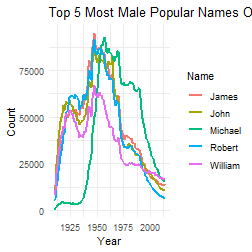
\includegraphics{Question2_files/figure-latex/Figure2-1} 

}

\caption{Metallica Album Popularity \label{Figure2}}\label{fig:Figure2}
\end{figure}

To contextualize the musical evolution of Coldplay and Metallica within
broader music industry trends, supplementary data sources are utilized,
including the Billboard Top 100 charts spanning several decades. This
analysis involved comparing the attributes of Coldplay and Metallica's
tracks---such as tempo, energy, valence, danceability, and popularity
with trends observed in mainstream music over the years all of which is
represented in the line graphs below. This comparative approach allowed
for a deeper understanding of how Coldplay and Metallica's musical
progression aligns with or stands apart from the prevailing trends in
popular music, shedding light on their unique contributions to the
industry and their ability to adapt to or influence broader musical
movements.

\begin{figure}[H]

{\centering \includegraphics{Question2_files/figure-latex/Figure3-1} 

}

\caption{Evolution of Music over time \label{Figure3}}\label{fig:Figure3}
\end{figure}

Metallica shows fluctuating but overall high energy levels throughout
their career. Coldplay started of their careers making more melow music
but shows a rising trend in energy over the years, indicating a shift
towards more energetic music in their later works.

Valence for both bands shows interesting trends. Metallica generally has
a lower valence compared to Coldplay, likely due to the subject matter
of some of their songs. Coldplay's valence has varied but shows a slight
upward trend, indicating more positive or emotionally uplifting music in
recent years.

Metallica maintains a lower danceability score throughout their career
but given that they primarily produce thrash metal this is consistent
with their genre and style. Coldplay's danceability shows an increasing
trend, aindicating a move towards more pop and rhythm-oriented music in
recent albums.

Both bands exhibit changes in song duration over the years. Metallica's
song durations have seen more fluctuation but they generally tend to be
much longer than that of Coldplay. However, Coldplay's songs have seen
an increase in duration over time, possibly refelcting more complex song
structures or varied musical explorations.

Compared to the Billboard 100, Metallica's music stands out with higher
energy and lower valence, emphasizing their thrash metal identity while
Coldplay's musical progression aligns more closely with mainstream
trends, showing increasing energy and danceability, possibly explaining
their more consistent levels popularity.

The heat maps below provide further insights into how different each
bands musical elements relate to each other within their discography.
This analysis contextualizes the distinctive musical characteristics and
evolution of Metallica and Coldplay over time, highlighting their
genre-specific traits and potential shifts in musical style and approach
across their careers.

\begin{figure}[H]

{\centering \includegraphics{Question2_files/figure-latex/Figure4-1} 

}

\caption{Heatmap of Metallicas musical attributes\label{Figure4}}\label{fig:Figure4}
\end{figure}

For Metallica, we see that loudness and energy are highly positively
correlated, as are acousticness and liveness. On the other hand,
danceability and acousticness, danceability and loudness, and
instrumentalness and valence have notable negative correlations.This
suggests that Metallica's loud and energetic music tends to be less
danceable and less acoustic.

\begin{figure}[H]

{\centering \includegraphics{Question2_files/figure-latex/Figure5-1} 

}

\caption{Heatmap of Coldplays musical attributes\label{Figure5}}\label{fig:Figure5}
\end{figure}

For Coldplay, energy and loudness, and acousticness and valence all see
positive correlations while danceability and acousticness, and liveness
and acousticness see negative correlations. This indicates that
Coldplay's more energetic and loud songs tend to be less acoustic, and
there is a distinct separation between acoustic and danceable tracks.

\section{Conclusion}\label{conclusion}

In comparing Metallica and Coldplay, their contrasting musical journeys
highlight diverse paths to longevity and relevance in the music
industry. Metallica has remained steadfast in their heavy metal roots,
maintaining a high-energy profile while adapting their sound within the
constraints of their genre. Over their career, they've shown
fluctuations in popularity, with early albums experiencing peaks. In
contrast, Coldplay has demonstrated a more adaptive style, evolving from
softer alternative rock to incorporating energetic and danceable
elements, aligning with broader pop trends. Their consistent popularity
across their discography underscores their ability to evolve while
maintaining widespread appeal. Together, these bands exemplify how
artistic evolution and genre adaptation can sustain enduring success in
contemporary music.

\bibliography{Tex/ref}





\end{document}
